\chapter{Fluxgate Magnetometer Basics \& Applications}
\lhead{\emph{Fluxgate Magnetometer Basics \& Applications}}
\section{Basics}
Fluxgate sensors are solid-state devices used for measuring the magnitude and direction of dc or low-frequency ac magnetic fields. Fluxgate sensors come in several configurations, the ring core type being the most commonly used. The fuxgate sensor used for magnetic field measurements in
the active shielding system developed for this thesis is a racetrack  fluxgate, which is essentially a modification of the ring core type sensor. Figure A.1 shows the main components of a ring core  fluxgate sensor. The central ring is typically made from an alloy of high magnetic permeability \(\mu\), wrapped in two sets of coil windings. The first set of windings, which are wrapped directly around the ring, are known as the drive windings or the excitation coil. The second set of windings are wrapped around the entire ring forming a pick-up, or sense coil. An ac current is driven into the excitation coil inducing a magnetic  flux \(\phi\) within the core. This field from the excitation coil causes the core to become magnetically saturated. If the core is thought of as two separate halves, then a the field generated in one half \((\phi_1)\) will be in the opposite direction as a the field generated in the other half \((\phi_2)\). If no external magnetic field is present, the two half cores go in and out of saturation simultaneously. The fields generated by the two half cores cancel, and no net change in  flux is measured by the pick-up coil. If an external field B0 is present, it will cause the saturation in each half of the core to vary relative to one another. The fields produced by the half cores no longer cancel and the pick-up coil is subjected to a net  flux. The result is an induced voltage in the pick-up coil, which provides a measure of the external field.



The sensor can be placed in a feedback loop (as shown in Figure A.2) in which another coil,known as the compensation or feedback coil, is used to drive the external field to zero resulting in no voltage output from the pick-up coil. The feedback loop maintains the zero voltage output from the pick-up coil by adjusting the current in the feedback coil. The external field measurement is then based on the current driven into the feedback coil. This is known as a feedback magnetometer, and the benefit is an increase in the dynamic range of the  fluxgate field measurement \cite{flux1}.

\section{Applications}
\begin{enumerate}
   \item Airborne Magnetics.
   \begin{itemize}
     \item 
   \end{itemize}
   \item Archaeology.
   \begin{itemize}
     \item 
   \end{itemize}
   \item Forensics.
   \begin{itemize}
     \item 
   \end{itemize}
   \item Exploration.
   \begin{itemize}
     \item 
   \end{itemize}
   \item Geosciences.
   \begin{itemize}
     \item 
   \end{itemize}
   \item Industrial.
   \begin{itemize}
     \item 
   \end{itemize}
   \item Medical.
   \begin{itemize}
     \item 
   \end{itemize}
   \item Near Surface Geophysics.
   \begin{itemize}
     \item 
   \end{itemize}
   \item Physics.
   \begin{itemize}
     \item 
   \end{itemize}
\end{enumerate}




\section{Use of Filter}
For prototype active magnetic field compensation system, it is required to use low pass filter (LPF) to ignore high frequency noises coming out from fluxgate sensors.

\begin{figure*}[t]
    \centering
    \captionsetup{justification=centering,margin=1cm}
    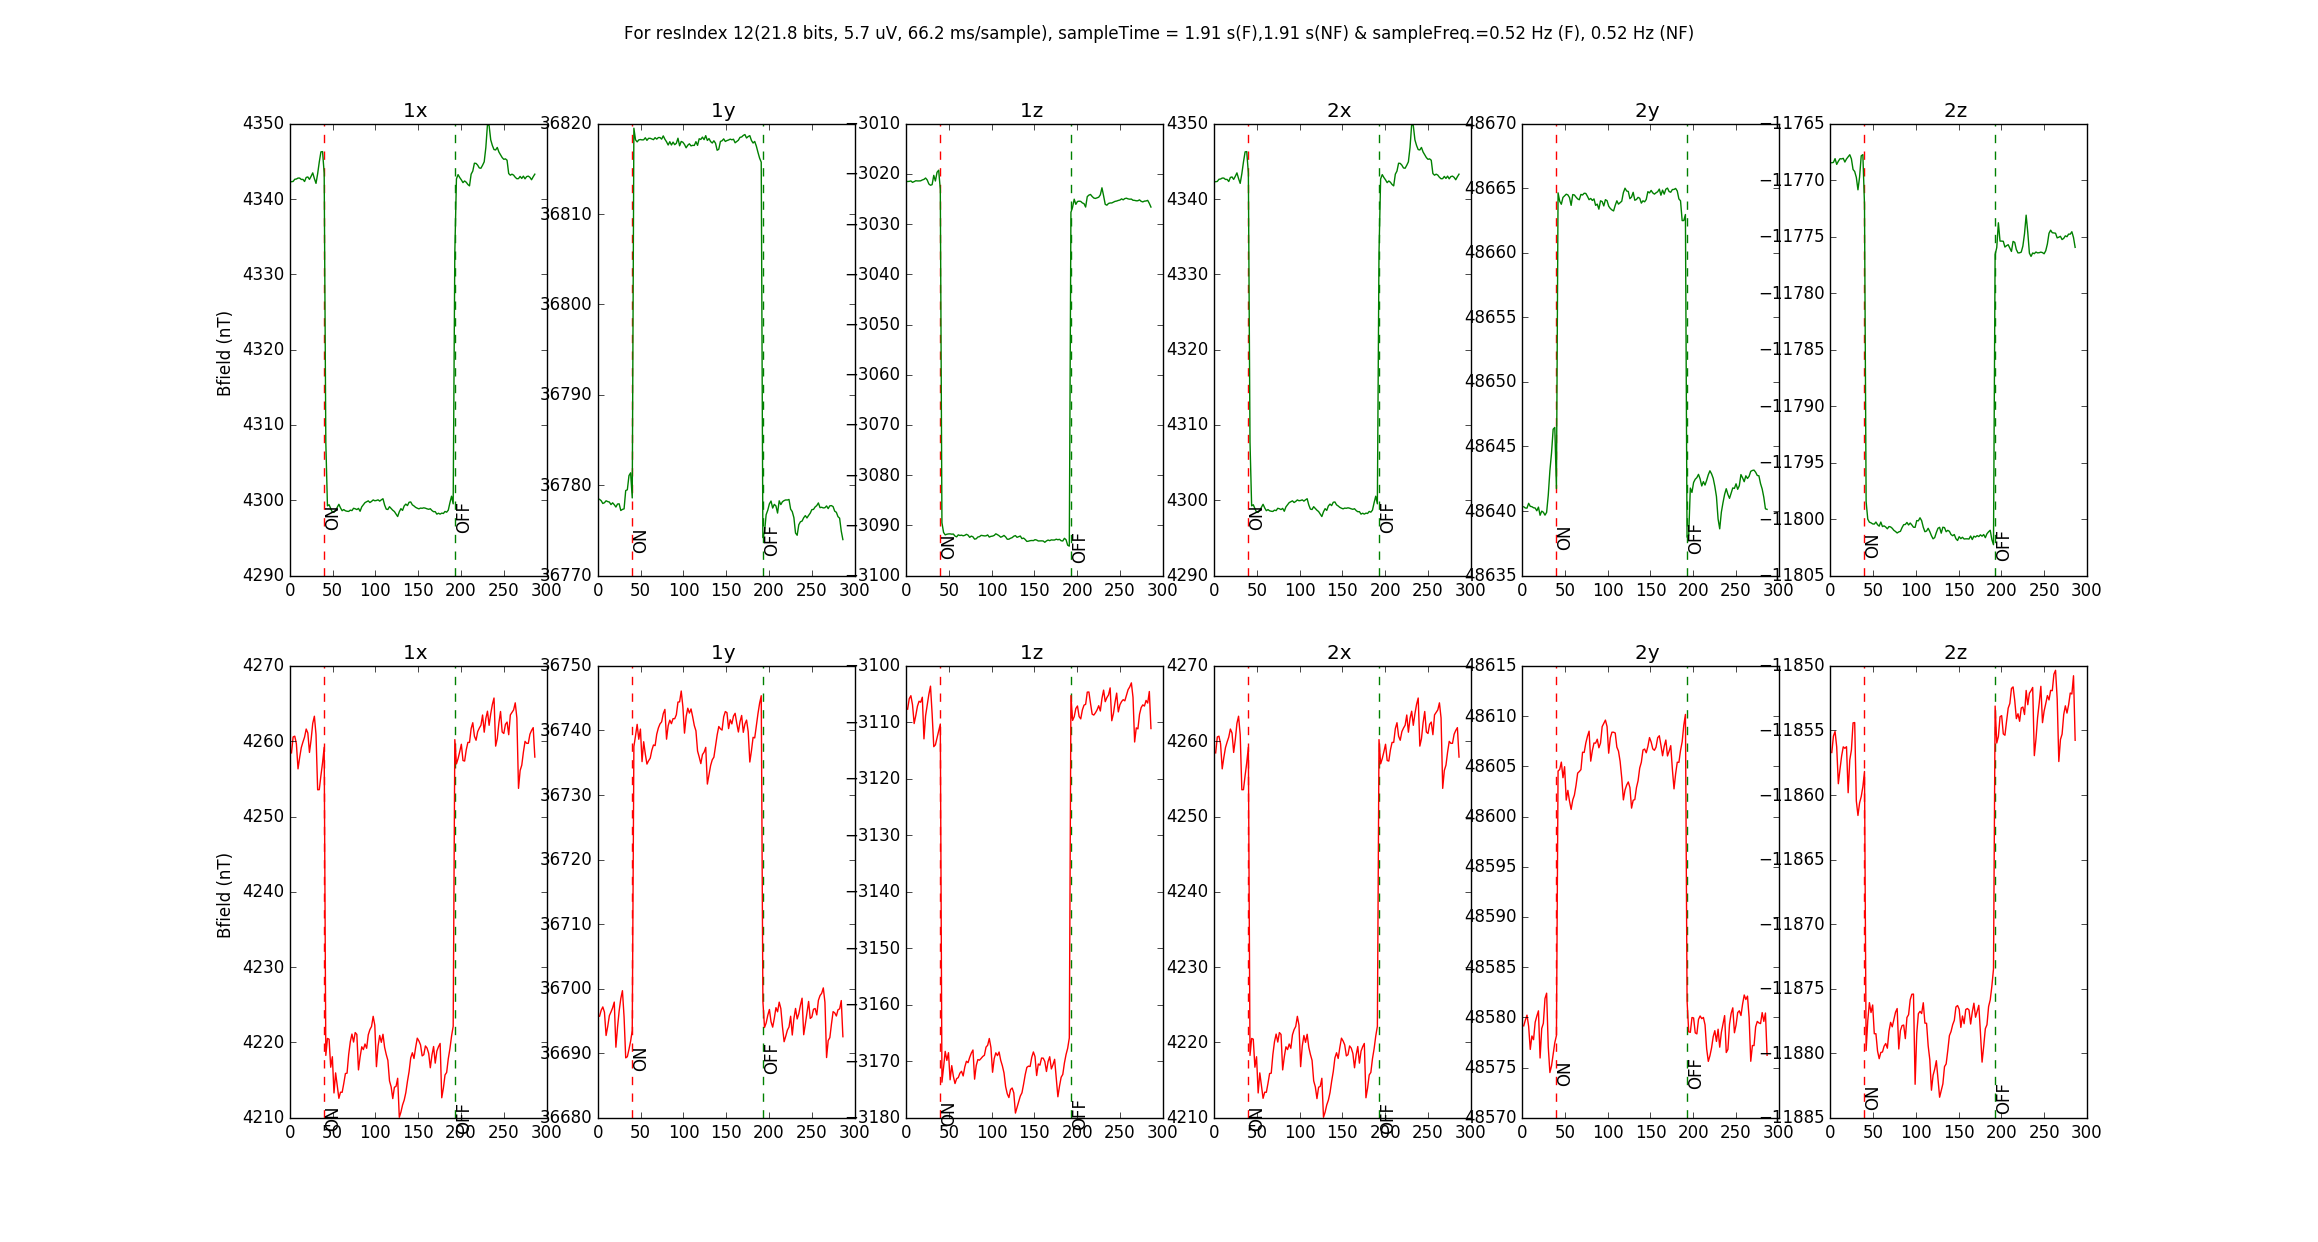
\includegraphics[height=3in, width=6in]{Figures/flux_r12.png}
    % \includegraphics[width=.80\textwidth]{socialDiscovery.eps}
    \caption{B field vs T for sample time 1.91 s\label{fig: fr12_1,2}}
\end{figure*}
For example, compensation can be done using 21.8 bits resolution. In that case, we don't need any filter as shown in the figure \ref{fig: fr12_1,2}.

But, for increasing the response of the feedback system, ADC resolution has to decrease which in turns introduce high frequency noise in the system that can be removed using LPF filter as shown in fig. \ref{fig: fr1_1,2} \& \ref{fig: fr8_1,2}. Thus , the sample time is vastly decreased by 96 times for fig. \ref{fig: fr8_1,2} and even more 191 times for fig. \ref{fig: fr1_1,2}.
\begin{figure*}[t]
    \centering
    \captionsetup{justification=centering,margin=1cm}
    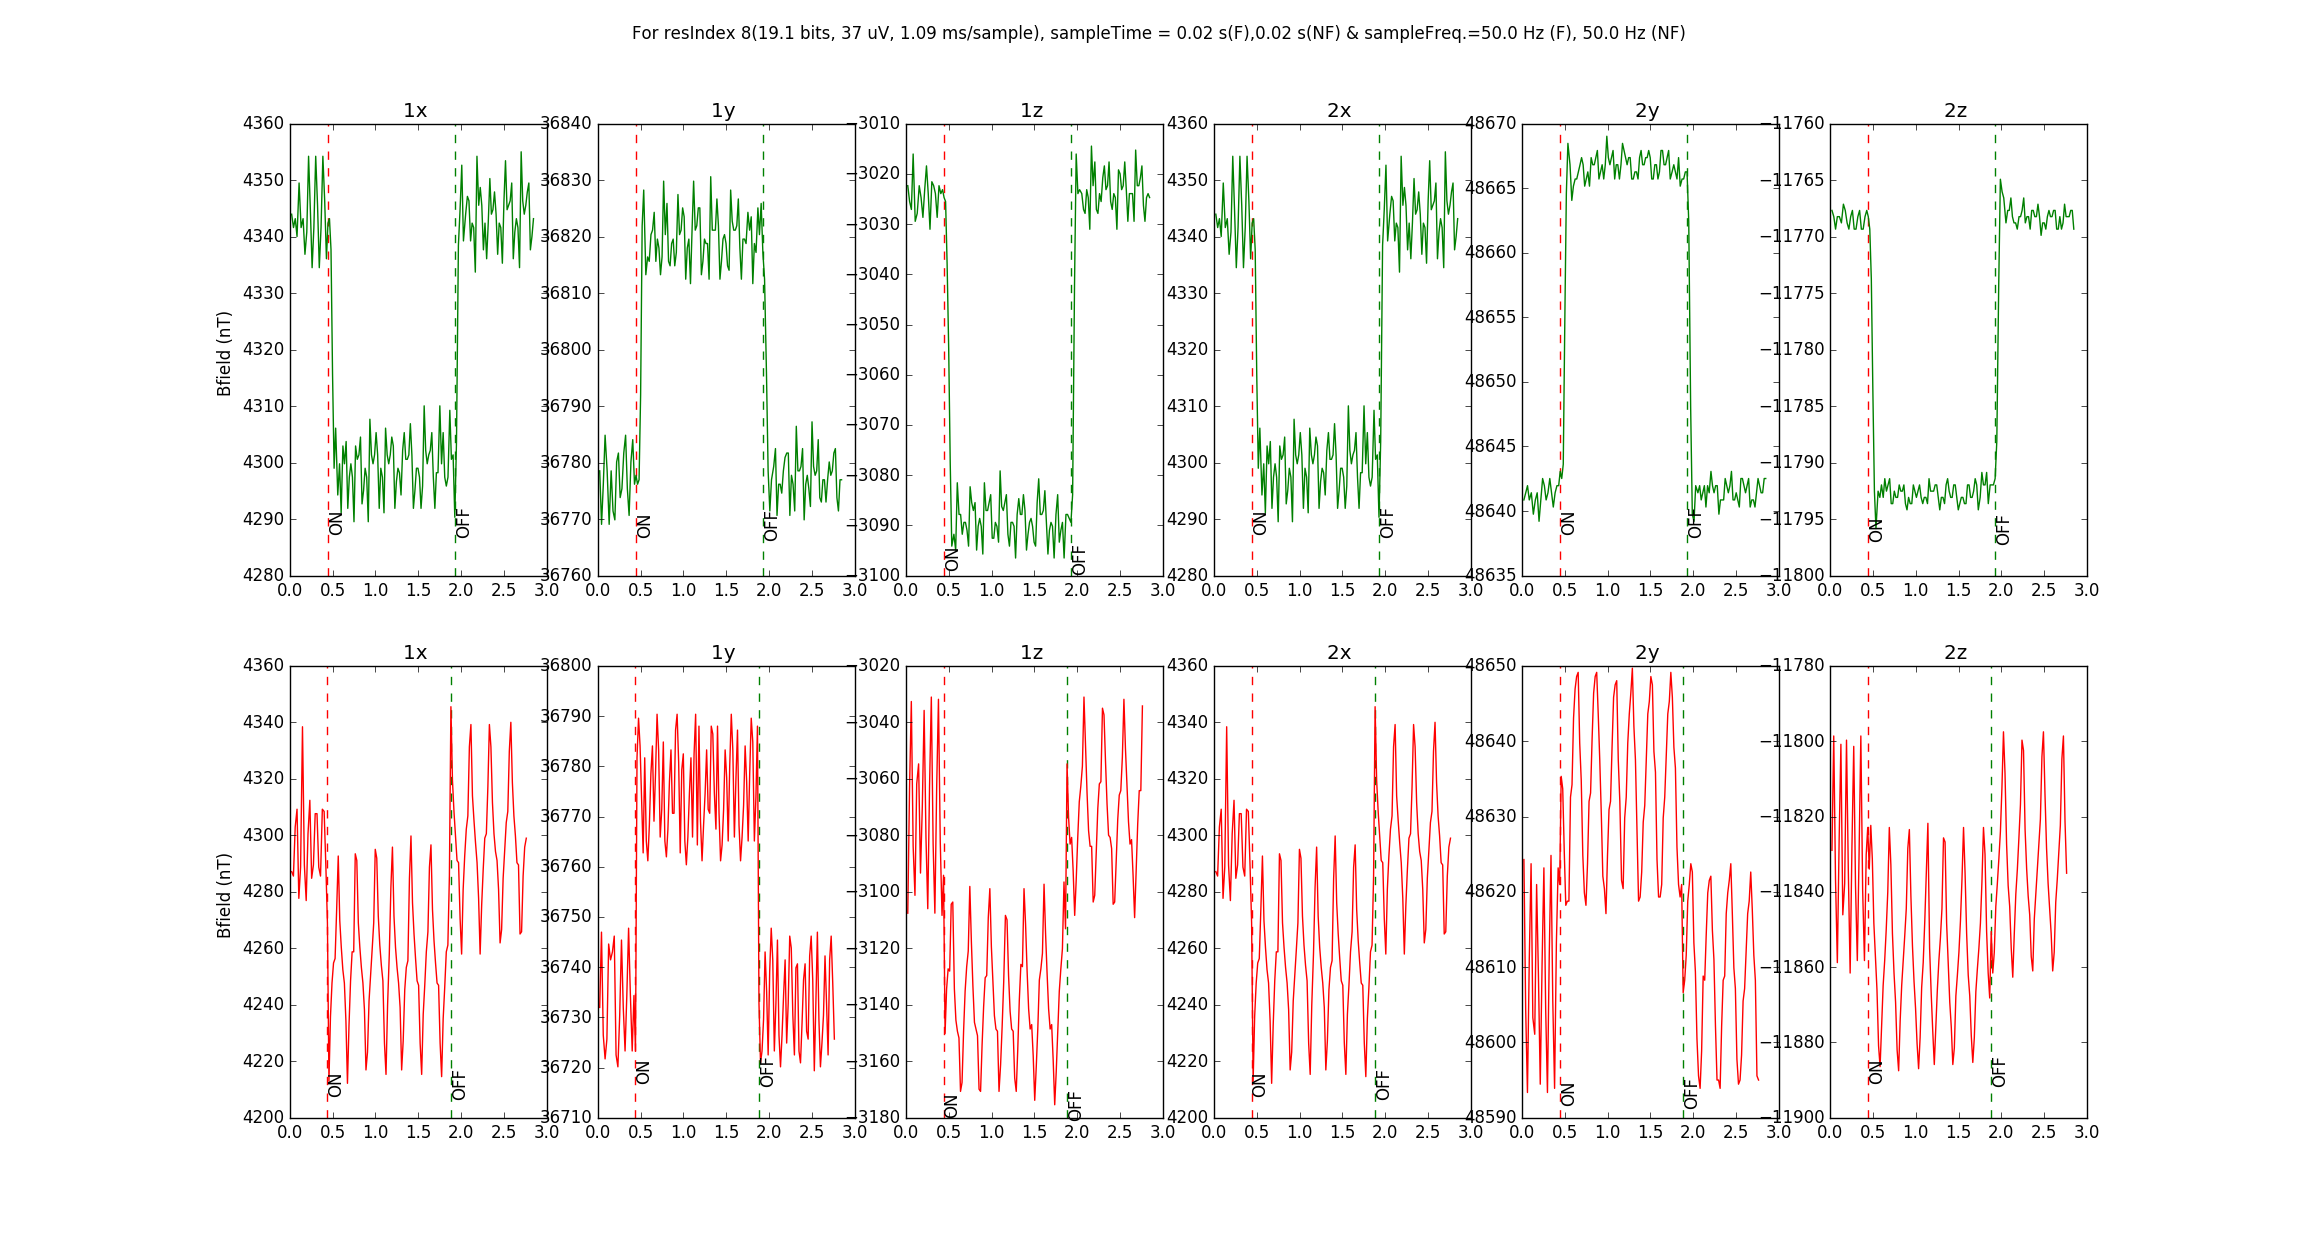
\includegraphics[height=3in, width=6in]{Figures/flux_r8.png}
    % \includegraphics[width=.80\textwidth]{socialDiscovery.eps}
    \caption{B field vs T for sample time 0.02 s\label{fig: fr8_1,2}}
\end{figure*}
\begin{figure*}[t]
    \centering
    \captionsetup{justification=centering,margin=1cm}
    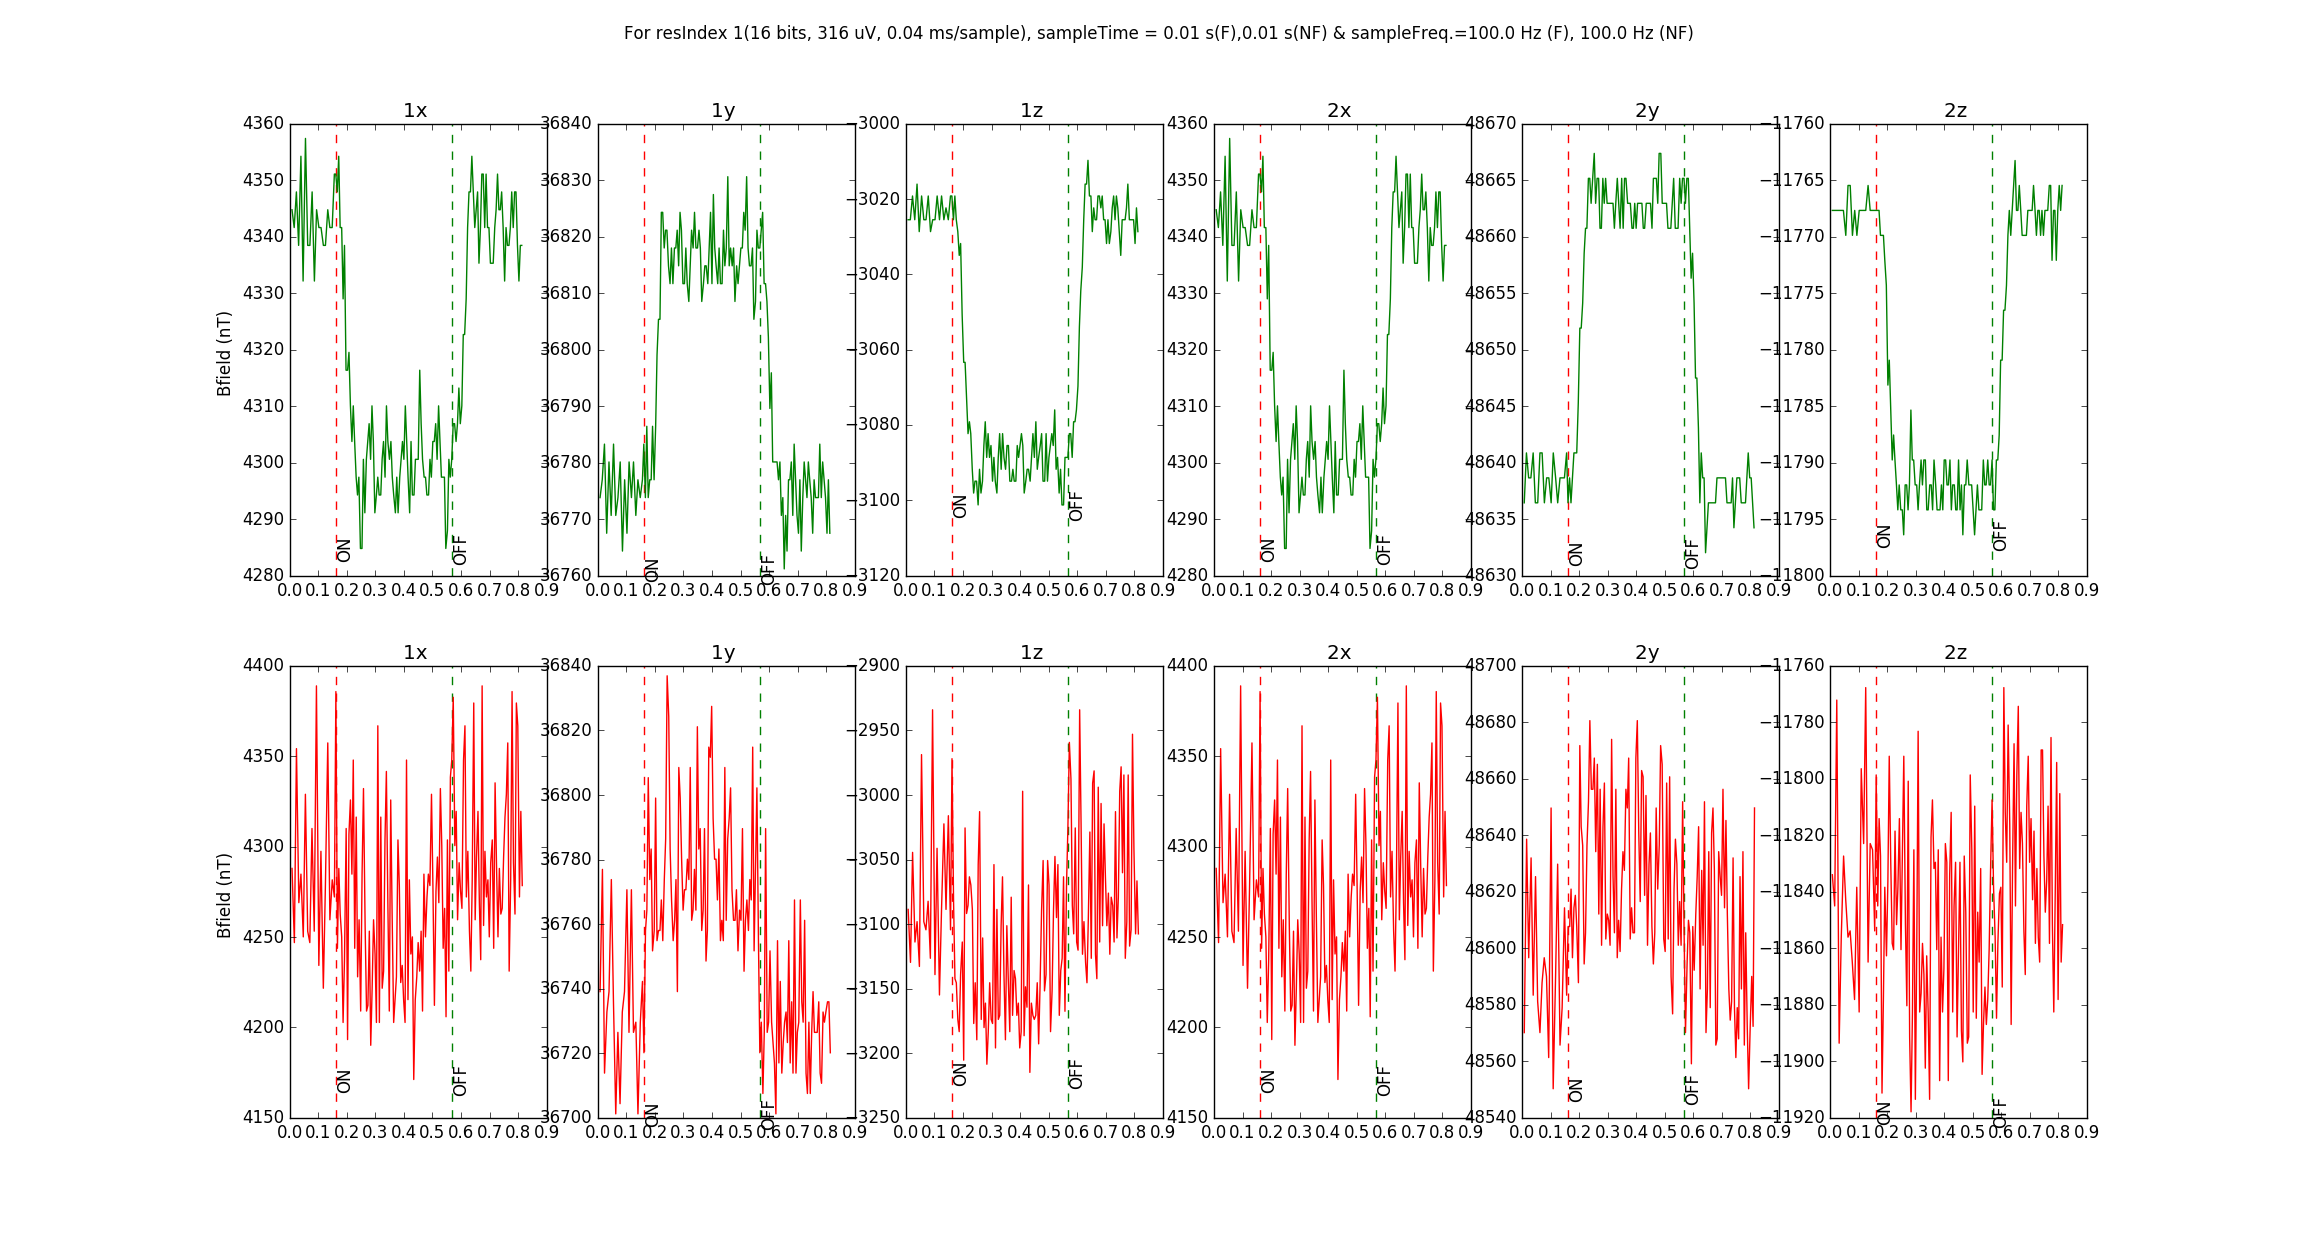
\includegraphics[height=3in, width=6in]{Figures/flux_r1.png}
    % \includegraphics[width=.80\textwidth]{socialDiscovery.eps}
    \caption{B field vs T for sample time 0.01 s\label{fig: fr1_1,2}}
\end{figure*}